\textbf{Constraint Programming} is really powerful when we have to deal within \textbf{scheduling problems}. Typically, such problems are described by the 
following definition.
\begin{definition}[title = Task scheduling definition]
    Schedule $n$ tasks on a machine, in time $D$, by obeying the temporal and precedence constraints:
    \begin{enumerate}
        \item Each task $t_i$ has a specific fixed processing time $p_i$.
        \item Each task $t_i$ can be started after its release date $r_i$ and must be completed before its deadline $d_i$.
        \item Tasks cannot overlap in time.
        \item Precedence relations must be respected.
    \end{enumerate}
\end{definition}
\begin{example}
    e.g. Task scheduling general problem. \vspace{7pt}

    Before we get into the solution, let's take a look at the image below. \vspace{3.5pt}
    \begin{center}
        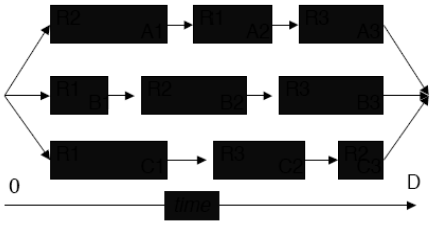
\includegraphics[width = 0.5\textwidth]{img/img5.png}
    \end{center} \vspace{3.5pt}
    Observing the figure, we can state:
    \begin{itemize}
        \renewcommand{\labelitemi}{-}
        \item Every black box is a task $t_i$ and its size determines the fixed processing time $p_i$.
        \item Every flow does not overlap tasks in the same row.
        \item Every flow respects the precedence relationships. 
    \end{itemize} \vspace{7pt}

    We could express decision variables, domains and constraints of any kind of task scheduling problem following a generic approach. \vspace{7pt}

    \textbf{Generic approach}. \\
    Since the more interisting part of the optimization problem is the starting time of tasks $t_i$, the same decision variables can be directly described as the starting time;
    this is possible since we already know how much time any process requires. \vspace{7pt}

    \textbf{Decision variables and domains}. \\
    We call $Start_i$ the decision variables representing the starting time of tasks $t_i$, where each of them takes a value from $[0 \dots D]$. \vspace{7pt}

    The domain $[0 \dots D]$ defines all the time we have available to compute our tasks $t_i$. \vspace{7pt}

    \textbf{Constraints}.
    \begin{itemize}
        \renewcommand{\labelitemi}{-}
        \item Respect of release date and deadline. 
        \begin{itemize}
            \item $\text{for all } i \in \{1, \dots, n\} \text{ such that } r_i \leq Start_i \leq d_i - p_i$ \\
            where: 
            \begin{itemize}
                \item $r_i \rightarrow$ release time
                \item $d_i \rightarrow$ deadline time
                \item $p_i \rightarrow$ processing time
                \item $Start_i \rightarrow$ starting time of the task $t_i$
            \end{itemize}
        \end{itemize}
        \item No overlap in time. 
        \begin{itemize}
            \item $\text{for all } i < j \text{ } \in \{1, \dots, n\} \text{ such that } (Start_i + p_i \leq Start_j) \vee (Start_j + p_j \leq Start_i)$ \\
            where:
            \begin{itemize}
                \item $p_i \rightarrow$ processing time of the task $t_i$
                \item $p_j \rightarrow$ processing time of the task $t_j$
                \item $Start_i \rightarrow$ starting time of the task $t_i$
                \item $Start_j \rightarrow$ starting time of the task $t_j$
            \end{itemize}
        \end{itemize}
        \item Precedence constraints. 
        \begin{itemize}
            \item $Start_i + p_i \leq Start_j \text{ for each pair of tasks } t_i \mapsto t_j$ \\
            where:
            \begin{itemize}
                \item $p_i \rightarrow$ processing time of the task $t_i$
                \item $Start_i \rightarrow$ starting time of the task $t_i$
                \item $Start_j \rightarrow$ starting time of the task $t_j$
                \item $t_i \mapsto t_j \rightarrow$ precedence relation between tasks $t_i$ and $t_j$
            \end{itemize}
        \end{itemize}
    \end{itemize} \vspace{7pt}

    \textbf{Final mark}. \\
    Before moving on, let's take a look at the final two constraints.
    \begin{itemize}
        \renewcommand{\labelitemi}{}
        \item $2^{nd}$ No overlap in time. \\ The starting and ending time of any pair of tasks ($t_i$, $t_j$) must be either the same time or ordered time, but they are never allowed to overlap each other.
        \item $3^{rd}$ Precedence constraints. \\ In almost of the cases, the second part of the previous constraint doesn't even exist (\textit{$\vee \text{ } (Start_j + p_j \leq Start_i)$}), since in general the output of a task it's used by another task as input, relying on the precedence relationships.
    \end{itemize}
\end{example}